\documentclass{article}

\usepackage{apacite}
\usepackage[table,xcdraw]{xcolor} % Color the table
\usepackage{parskip} % Disable the second and onward paragraph indentation
\usepackage{listings} % Code Snippets
\lstset{language=Python}
\usepackage{float} % \begin{table}[H] To avoid table repositioning
\usepackage{graphicx} % Insert images
\usepackage{subcaption}
%\graphicspath{ {./Images/} }

\renewcommand{\arraystretch}{1.5} 		% Adjust rows' height in table

\title	{Confronto della Performance degli Algoritmi di Ordinamento tra Raspberry Pi 3 e Personal Computer}
\author	{Marco De Groskovskaja}
\date	{\today}

\usepackage [
	a4paper,
	left=3cm,
	right=3cm,
	top=3cm,
	bottom=3cm,
] {geometry}

\begin{document}
	\maketitle
	
	\section{Introduzione}
		
		Questa relazione esplora le differenze di performance tra il Raspberry Pi 3 model B+ e il Personal Computer Lenovo Thinkbook 15 G3 ACL per gli algoritmi di ordinamento: BubbleSort, InsertionSort, MergeSort e QuickSort.
	
	\section{Presentazione delle piattaforme}
		\subsection{Raspberry Pi 3 model B+}
			\begin{minipage}{0.6\textwidth}\raggedright
				\textbf{Processore:}
				\hspace{1mm} Broadcom BCM2837B0, Cortex-A53
				\newline
				\newline
				\textbf{Memoria:}
				\hspace{4mm} 1GB LPDDR2 SDRAM
				\newline
				\newline
				\textbf{SO:}
				\hspace{15mm} Raspberry Pi OS
			\end{minipage}
			\begin{minipage}{0.3\textwidth}
				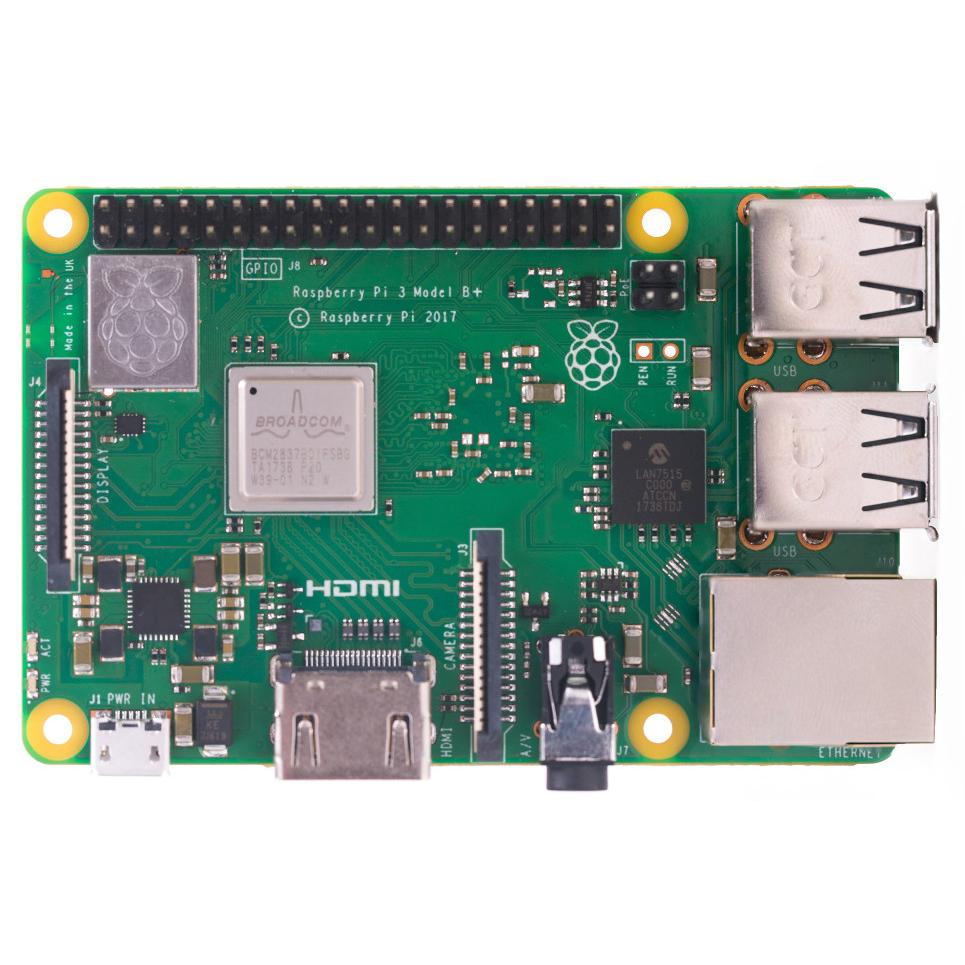
\includegraphics[width=\linewidth]{./Imgs/RaspberryBoard.jpg}
			\end{minipage}

		\subsection{Lenovo Thinkbook 15 G3 ACL}
			\begin{minipage}{0.6\textwidth}\raggedright
				\textbf{Processore:}
				\hspace{1mm} AMD Ryzen™ 5 5500U
				\newline
				\newline
				\textbf{Memoria:}
				\hspace{4mm} 16 GB DDR4 2400MHz
				\newline
				\newline
				\textbf{SO:}
				\hspace{15mm} Windows 10 Pro
			\end{minipage}
			\begin{minipage}{0.3\textwidth}
				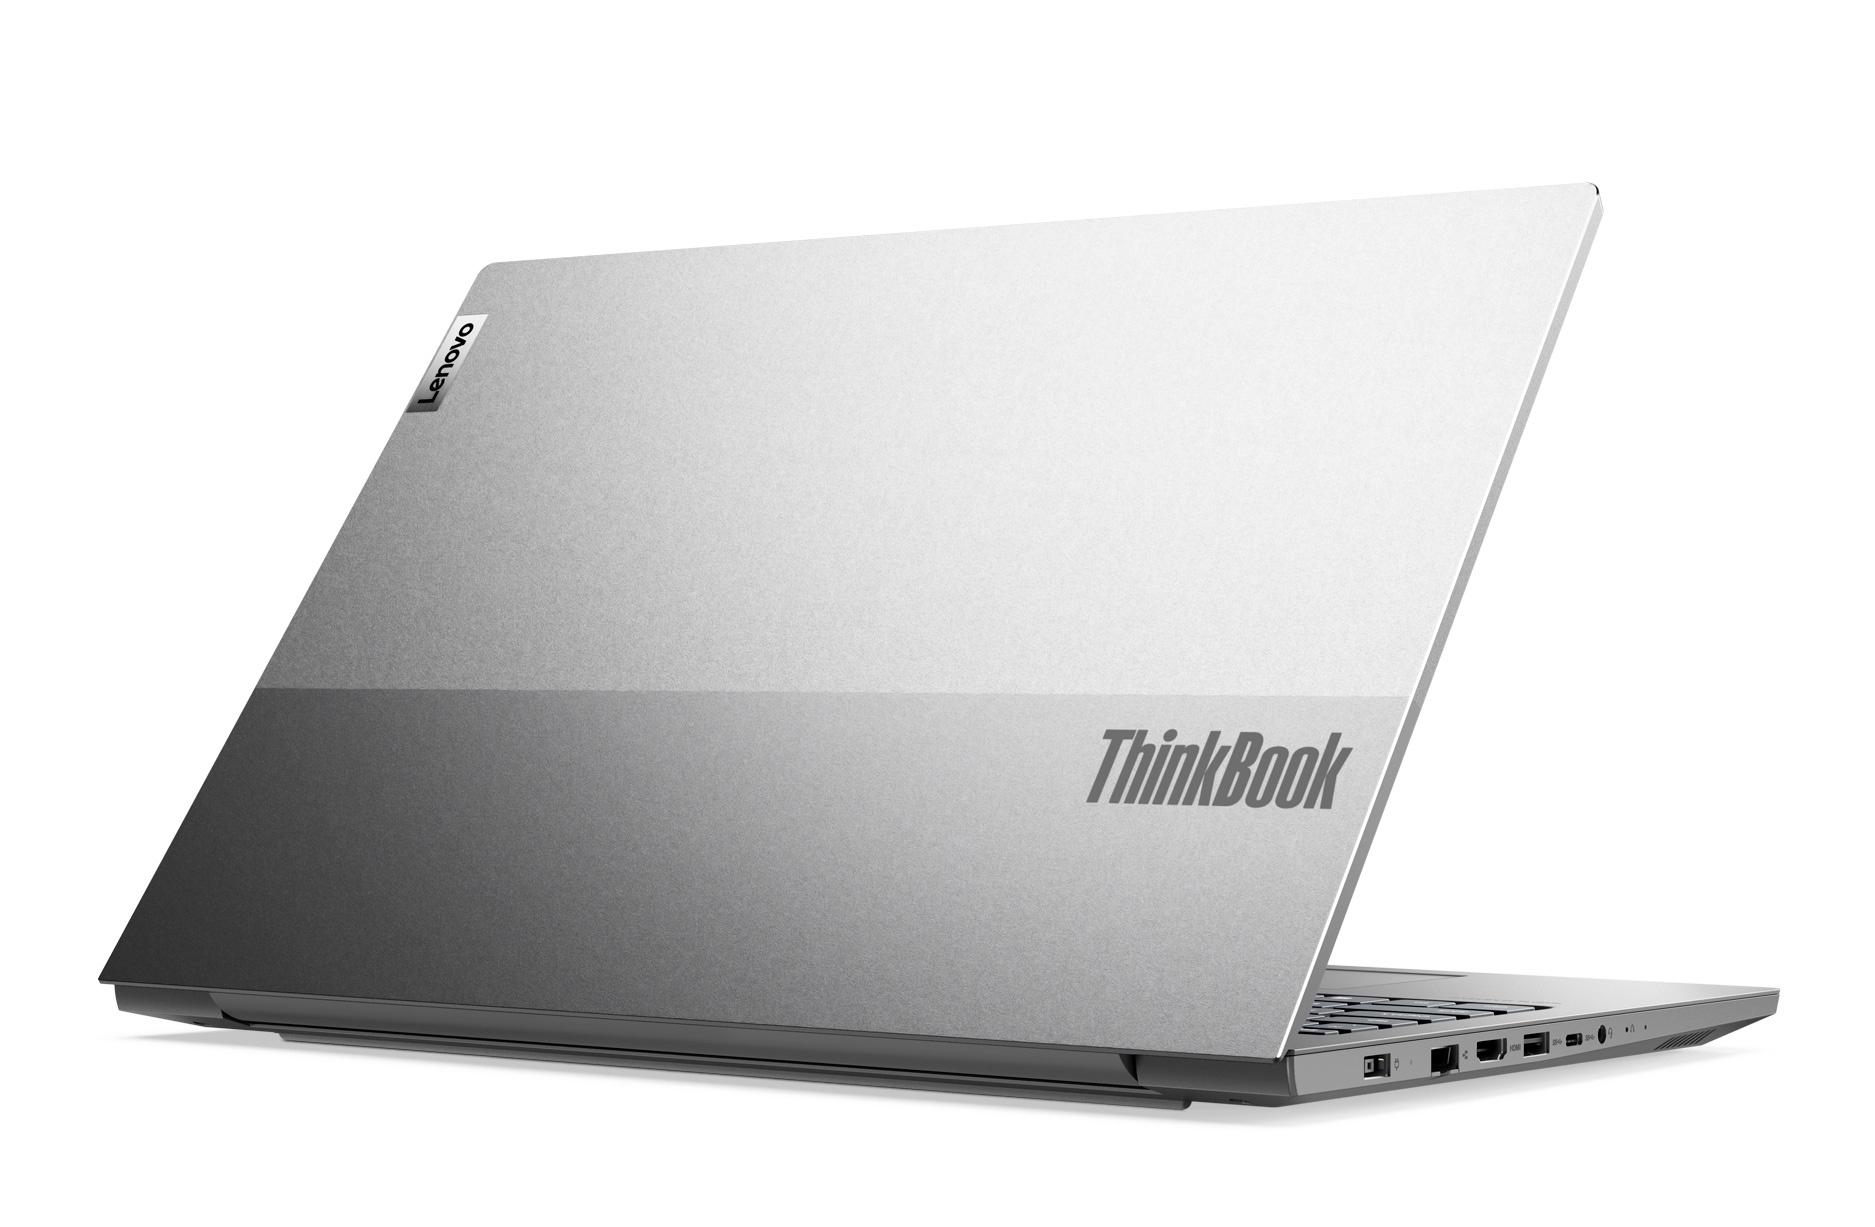
\includegraphics[width=\linewidth]{./Imgs/PersonalComputer.jpg}
			\end{minipage}
		
	\newpage
	\section{1° Algoritmo di Ordinamento: \textit{BubbleSort}}
		\subsection{Introduzione}
			Bubble Sort è un algoritmo di ordinamento molto semplice ma inefficace per grandi quantità di dati. L'idea di base di Bubble Sort è di confrontare coppie di elementi adiacenti in un elenco e scambiare i loro valori se non sono in ordine. L'algoritmo esegue questo confronto e scambio di valori in modo ripetuto, finché l'intero elenco non è ordinato.
			
			Ecco come funziona Bubble Sort in dettaglio:
			\begin{enumerate}
				\item L'algoritmo inizia dal primo elemento dell'elenco e confronta il valore di questo elemento con il valore del secondo elemento. Se il primo elemento è maggiore del secondo, i due elementi vengono scambiati.
				
				\item  L'algoritmo procede quindi a confrontare il secondo e il terzo elemento e così via, fino alla fine dell'elenco.
				
				\item Alla fine del primo passaggio, l'ultimo elemento dell'elenco conterrà il valore più grande.
				
				\item L'algoritmo quindi ripete il processo, confrontando coppie di elementi adiacenti e scambiandoli se necessario, fino a quando l'elenco intero è stato ordinato.
			\end{enumerate}
		
		\subsection{Complessità Algoritmica}
			I limiti asintotici della complessità temporale previsti per l' algoritmo di ordinamento BubbleSort, sono i seguenti:

			\begin{table}[ht]
				\centering
				\begin{tabular}{|l|ccc|}
					\rowcolor[HTML]{C0C0C0}
					\hline
					Algoritmo    		& Caso Peggiore & Caso Medio & Caso Migliore \\
					\hline
					BubbleSort       	& O(n\textsuperscript{2})          & O(n\textsuperscript{2})    & O(n)          \\
					\hline
				\end{tabular}
				\caption{Complessità Temporale dell' algoritmo di ordinamento BubbleSort}
			\end{table}
		
		\subsection{Implementazione software}
			L'implementazione software dell' algoritmo di ordinamento BubbleSort è descritta nei file Python \textbf{\textit{BubbleSort.py}} alla relazione allegato.

	
	\newpage
	\section{2° Algoritmo di Ordinamento: \textit{InsertionSort}}
		\subsection{Introduzione}
			Insertion Sort è un algoritmo di ordinamento semplice ed efficiente per piccoli elenchi di elementi. L'idea di base di Insertion Sort è di considerare l'elenco come diviso in due parti: una parte ordinata e una parte non ordinata. L'algoritmo procede a inserire ogni elemento nella sua posizione corretta nella parte ordinata, spostando gli elementi di valore maggiore verso destra per fare spazio.
			
			Ecco come funziona Insertion Sort in dettaglio:
			\begin{enumerate}
				\item L'algoritmo inizia considerando il primo elemento dell'elenco come parte ordinata.
				
				\item L'algoritmo quindi procede a inserire il secondo elemento nella parte ordinata, confrontandolo con il primo elemento e spostando il primo elemento a destra se il secondo elemento è più piccolo.
				
				\item L'algoritmo quindi procede a inserire il terzo elemento nella parte ordinata, confrontandolo con il secondo elemento e il primo elemento e spostando gli elementi a destra se necessario.
				
				\item L'algoritmo continua a inserire ogni elemento successivo nella parte ordinata, spostando gli elementi di valore maggiore a destra per fare spazio, fino a quando l'elenco intero è stato ordinato.
			\end{enumerate}
		
		\subsection{Complessità Algoritmica}
			I limiti asintotici della complessità temporale previsti per l' algoritmo di ordinamento InsertionSort, sono i seguenti:
			
			\begin{table}[ht]
				\centering
				\begin{tabular}{|l|ccc|}
					\rowcolor[HTML]{C0C0C0}
					\hline
					Algoritmo    		& Caso Peggiore & Caso Medio & Caso Migliore \\
					\hline
					InsertionSort       	& O(n\textsuperscript{2})          & O(n\textsuperscript{2})    & O(n)          \\
					\hline
				\end{tabular}
				\caption{Complessità Temporale dell' algoritmo di ordinamento InsertionSort}
			\end{table}

		\subsection{Implementazione software}
			L'implementazione software dell' algoritmo di ordinamento InsertionSort è descritta nei file Python \textbf{\textit{InsertionSort.py}} alla relazione allegato.
		
	\newpage
	\section{3° Algoritmo di Ordinamento: \textit{MergeSort}}
		\subsection{Introduzione}
			Merge Sort è un algoritmo di ordinamento molto efficiente che utilizza una strategia di "divide et impera" per ordinare un elenco di elementi. L'algoritmo divide ripetutamente l'elenco in due parti, le ordina separatamente e poi le combina per produrre l'elenco ordinato finale.
			
			Ecco come funziona Merge Sort in dettaglio:
			\begin{enumerate}
				\item L'algoritmo divide l'elenco originale in due parti di lunghezza quasi uguale.
				
				\item L'algoritmo quindi ordina separatamente le due parti dell'elenco utilizzando una chiamata ricorsiva a se stesso.
				
				\item L'algoritmo combina le due parti ordinate in un unico elenco ordinato. In questo processo, l'algoritmo confronta i primi elementi di entrambe le parti dell'elenco e inserisce l'elemento più piccolo nell'elenco ordinato. L'algoritmo poi procede a confrontare i successivi elementi e a inserirli nell'elenco ordinato, fino a quando non sono stati inseriti tutti gli elementi.
				
				\item L'algoritmo ripete i passaggi 1-3 su ciascuna delle due parti dell'elenco diviso, fino a quando l'intero elenco non è stato ordinato.
			\end{enumerate}

		\subsection{Complessità Algoritmica}
			I limiti asintotici della complessità temporale previsti per l' algoritmo di ordinamento MergeSort, sono i seguenti:
			
			\begin{table}[ht]
				\centering
				\begin{tabular}{|l|ccc|}
					\rowcolor[HTML]{C0C0C0}
					\hline
					Algoritmo    		& Caso Peggiore & Caso Medio & Caso Migliore \\
					\hline
					MergeSort       	& O(n log(n))          & O(n log(n))    & O(n log(n))          \\
					\hline
				\end{tabular}
				\caption{Complessità Temporale dell' algoritmo di ordinamento MergeSort}
			\end{table}
	
		\subsection{Implementazione software}
			L'implementazione software dell' algoritmo di ordinamento MergeSort è descritta nei file Python \textbf{\textit{MergeSort.py}} alla relazione allegato.
	
	\newpage
	\section{4° Algoritmo di Ordinamento: \textit{QuickSort}}
		\subsection{Introduzione}
			Quick Sort è un algoritmo di ordinamento molto efficiente che utilizza una strategia di "divide et impera" per ordinare un elenco di elementi. L'algoritmo sceglie un elemento come "pivot", divide l'elenco in due parti, una con elementi minori o uguali al pivot e una con elementi maggiori del pivot, e poi ordina separatamente le due parti.
			
			Ecco come funziona Quick Sort in dettaglio:
			\begin{enumerate}
				\item L'algoritmo sceglie un elemento dell'elenco come "pivot". Questo può essere fatto scegliendo l'elemento più a sinistra, più a destra o un elemento casuale dell'elenco.
				
				\item L'algoritmo quindi ripartisce l'elenco in due parti: una parte con elementi minori o uguali al pivot e una parte con elementi maggiori del pivot. Ciò viene fatto attraverso una scansione dell'elenco, spostando gli elementi minori o uguali al pivot a sinistra dell'elenco e gli elementi maggiori del pivot a destra.
				
				\item L'algoritmo ordina separatamente le due parti dell'elenco utilizzando una chiamata ricorsiva a se stesso. Ogni chiamata ricorsiva ordina un sottoinsieme dell'elenco, compreso tra il primo elemento e l'elemento immediatamente precedente o successivo del pivot.
				
				\item L'algoritmo ricombina le due parti dell'elenco in un unico elenco ordinato. Per fare ciò, l'algoritmo posiziona il pivot al centro dell'elenco, con tutti gli elementi minori o uguali al pivot a sinistra e tutti gli elementi maggiori del pivot a destra.
				
				\item L'algoritmo ripete i passaggi 1-4 per le due parti dell'elenco finché non viene ottenuto l'elenco ordinato completo.
			\end{enumerate}
		
		\subsection{Complessità Algoritmica}
			I limiti asintotici della complessità temporale previsti per l' algoritmo di ordinamento QuickSort, sono i seguenti:
			
			\begin{table}[ht]
				\centering
				\begin{tabular}{|l|ccc|}
					\rowcolor[HTML]{C0C0C0}
					\hline
					Algoritmo    		& Caso Peggiore & Caso Medio & Caso Migliore \\
					\hline
					QuickSort       	& O(n\textsuperscript{2})          & O(n log(n))    & O(n log(n))          \\
					\hline
				\end{tabular}
				\caption{Complessità Temporale dell' algoritmo di ordinamento QuickSort}
			\end{table}

		\subsection{Implementazione software}
			L'implementazione software dell' algoritmo di ordinamento QuickSort è descritta nei file Python \textbf{\textit{QuickSort.py}} alla relazione allegato.

	\newpage
	\section{Test degli algoritmi di ordinamento}
		Di seguito vengono riportati i grafici dei test eseguiti sull'implementazione software degli algoritmi di ordinamento BubbleSort, InsertionSort, MergeSort e QuickSort, attraverso l' unità di testing definita nel file Python \colorbox{lightgray}{TestUnit.py} ed eseguita da \colorbox{lightgray}{main.py}.
		
		I dati sulle performance degli algoritmi di ordinamento in questione, eseguiti sulla piattaforma \textbf{Raspberry Pi 3 B+} sono invece stati raccolti attraverso il programma Python \colorbox{lightgray}{main\_on\_raspberry.py} e salvati nella cartella \colorbox{lightgray}{Data} con il nome \textit{raspberry\_data}.
		
		I test sono stati eseguiti per una sequenza in input \textit{Randomized}.
		
		Il numero di test eseguiti per ogni algoritmo di ordinamento è \textbf{\textit{m} = 300}, ciascuno dei quali su un array di dimensione variabile pari al numero del test, per esempio il primo test è stato esequito su un array di dimensione uno, il secondo test è stato eseguito su un array di dimensione due, e così via.

		\newpage
		\subsection{Test di BubbleSort}

			\begin{figure}[h!]
				\centering
				
				\begin{subfigure}{0.6\textwidth}
					\centering
					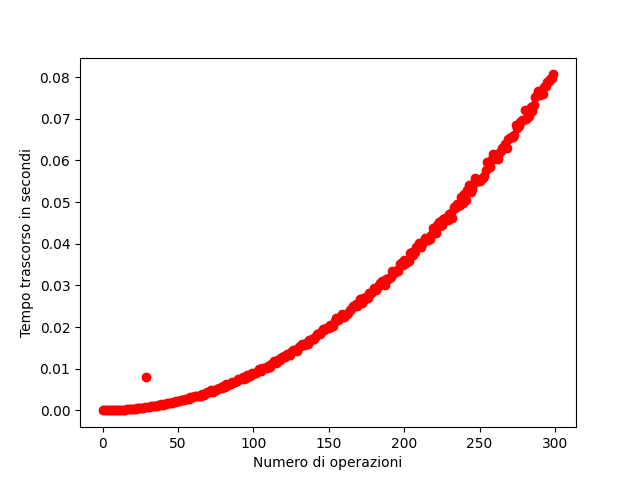
\includegraphics[width = \textwidth]{./Plots/Raspberry_BubbleSort.png}
					\caption{BubbleSort su Raspberry}
				\end{subfigure}
				\begin{subfigure}{0.6\textwidth}
					\centering
					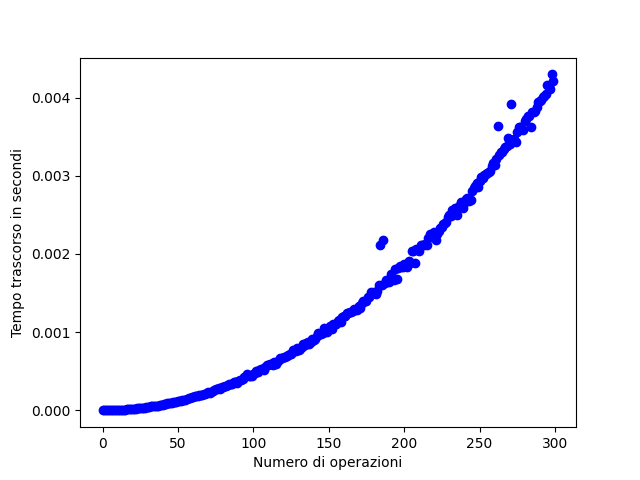
\includegraphics[width = \textwidth]{./Plots/Pc_BubbleSort.png}
					\caption{BubbleSort su Pc}
				\end{subfigure}
				\begin{subfigure}{0.6\textwidth}
					\centering
					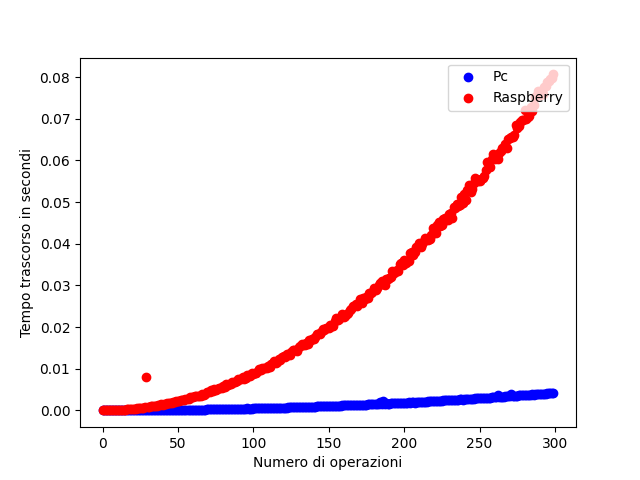
\includegraphics[width = \textwidth]{./Plots/PcVsRaspberry_BubbleSort.png}
					\caption{Raspberry Vs Pc}
				\end{subfigure}

			\end{figure}

		\clearpage
		\subsection{Test di InsertionSort}

			\begin{figure}[h!]
				\centering
				
				\begin{subfigure}{0.6\textwidth}
					\centering
					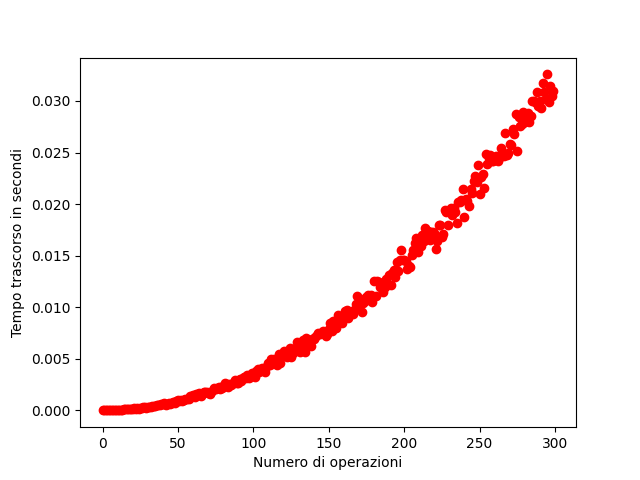
\includegraphics[width = \textwidth]{./Plots/Raspberry_InsertionSort.png}
					\caption{InsertionSort su Raspberry}
				\end{subfigure}
				\begin{subfigure}{0.6\textwidth}
					\centering
					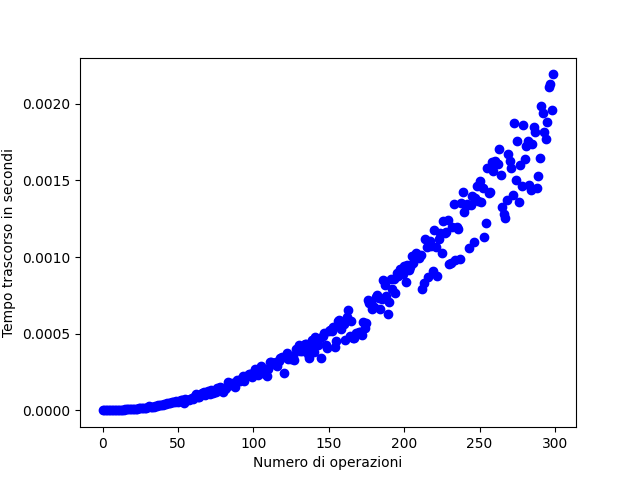
\includegraphics[width = \textwidth]{./Plots/Pc_InsertionSort.png}
					\caption{InsertionSort su Pc}
				\end{subfigure}
				\begin{subfigure}{0.6\textwidth}
					\centering
					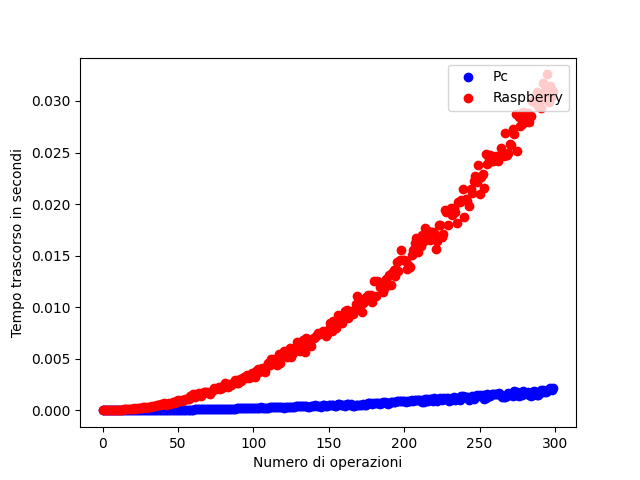
\includegraphics[width = \textwidth]{./Plots/PcVsRaspberry_InsertionSort.png}
					\caption{Raspberry Vs Pc}
				\end{subfigure}
				
			\end{figure}
	
		\clearpage
		\subsection{Test di MergeSort}

			\begin{figure}[h!]
				\centering
				
				\begin{subfigure}{0.6\textwidth}
					\centering
					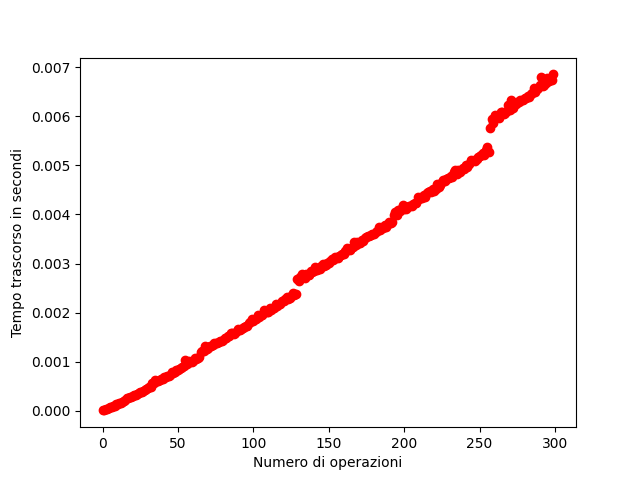
\includegraphics[width = \textwidth]{./Plots/Raspberry_MergeSort.png}
					\caption{MergeSort su Raspberry}
				\end{subfigure}
				\begin{subfigure}{0.6\textwidth}
					\centering
					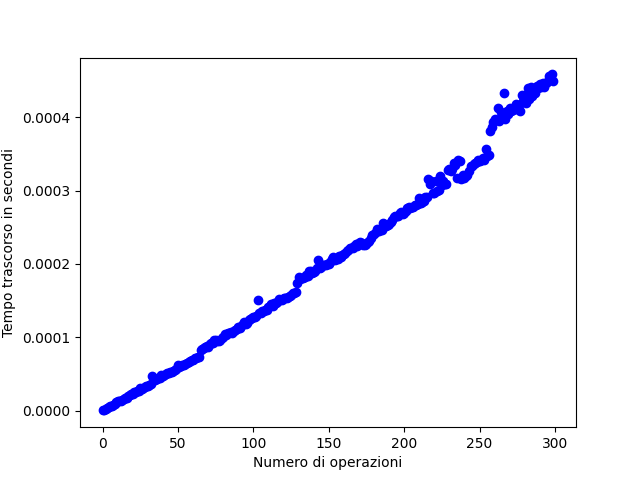
\includegraphics[width = \textwidth]{./Plots/Pc_MergeSort.png}
					\caption{MergeSort su Pc}
				\end{subfigure}
				\begin{subfigure}{0.6\textwidth}
					\centering
					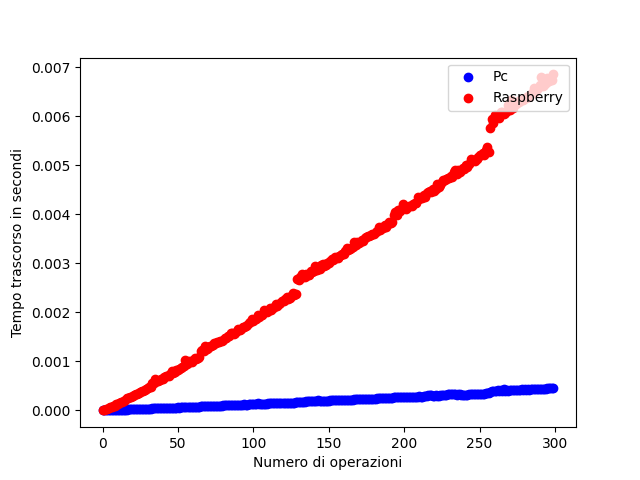
\includegraphics[width = \textwidth]{./Plots/PcVsRaspberry_MergeSort.png}
					\caption{Raspberry Vs Pc}
				\end{subfigure}
				
			\end{figure}
		
		\clearpage
		\subsection{Test di QuickSort}

			\begin{figure}[h!]
				\centering
				
				\begin{subfigure}{0.6\textwidth}
					\centering
					\includegraphics[width = \textwidth]{./Plots/Raspberry_QuickSort.png}
					\caption{QuickSort su Raspberry}
				\end{subfigure}
				\begin{subfigure}{0.6\textwidth}
					\centering
					\includegraphics[width = \textwidth]{./Plots/Pc_QuickSort.png}
					\caption{QuickSort su Pc}
				\end{subfigure}
				\begin{subfigure}{0.6\textwidth}
					\centering
					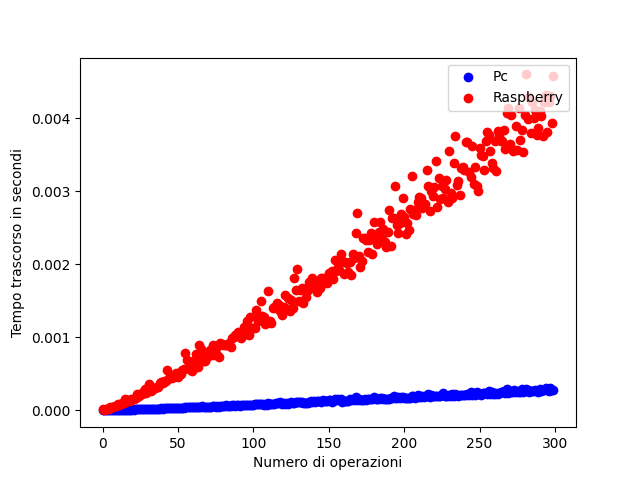
\includegraphics[width = \textwidth]{./Plots/PcVsRaspberry_QuickSort.png}
					\caption{Raspberry Vs Pc}
				\end{subfigure}
				
			\end{figure}
		
		\clearpage
		\subsection{Plots Combinati}
		
			\begin{figure}[h]
				\centering
				
				\begin{subfigure}{0.75\textwidth}
					\centering
					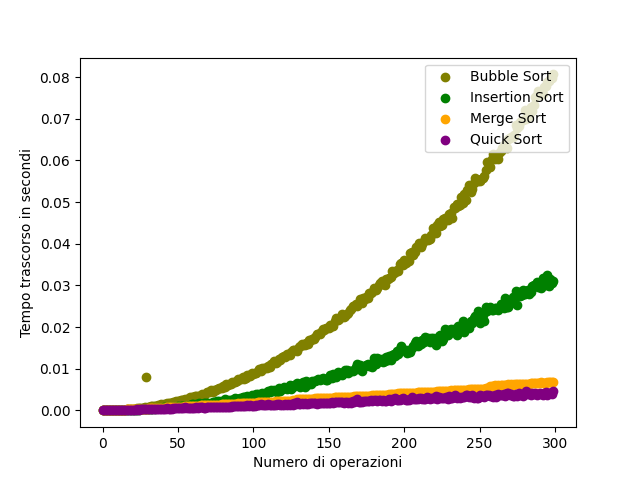
\includegraphics[width = \textwidth]{./Plots/Raspberry_CombinedTimestamps.png}
					\caption{Grafici combinati su Raspberry}
				\end{subfigure}
				\begin{subfigure}{0.75\textwidth}
					\centering
					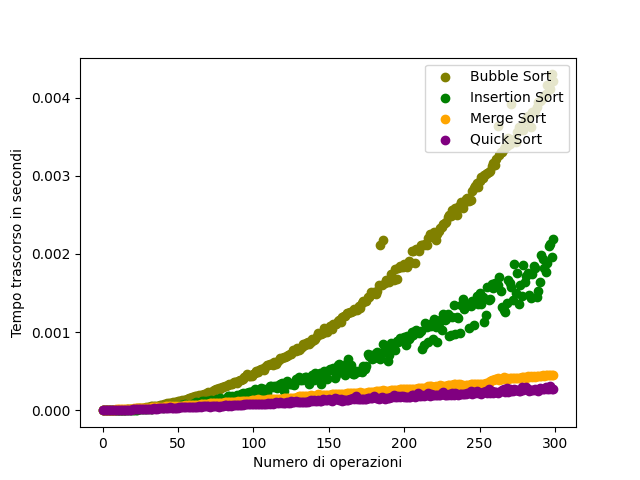
\includegraphics[width = \textwidth]{./Plots/Pc_CombinedTimestamps.png}
					\caption{Grafici combinati su pc}
				\end{subfigure}

			\end{figure}
	
		\clearpage
	\section{Conclusioni}
		I risultati dei test effettuati coincidono con la complessità attesa degli algoritmi di ordinamento in questione.
		È osservabile un grande aumento della performance degli algoritmi di ordinamento, quando eseguiti su Pc rispetto che sulla piattaforma Raspberry Pi 3 B+.
		
		\begin{figure}[h]
			\centering
			
			\begin{subfigure}{1\textwidth}
				\centering
				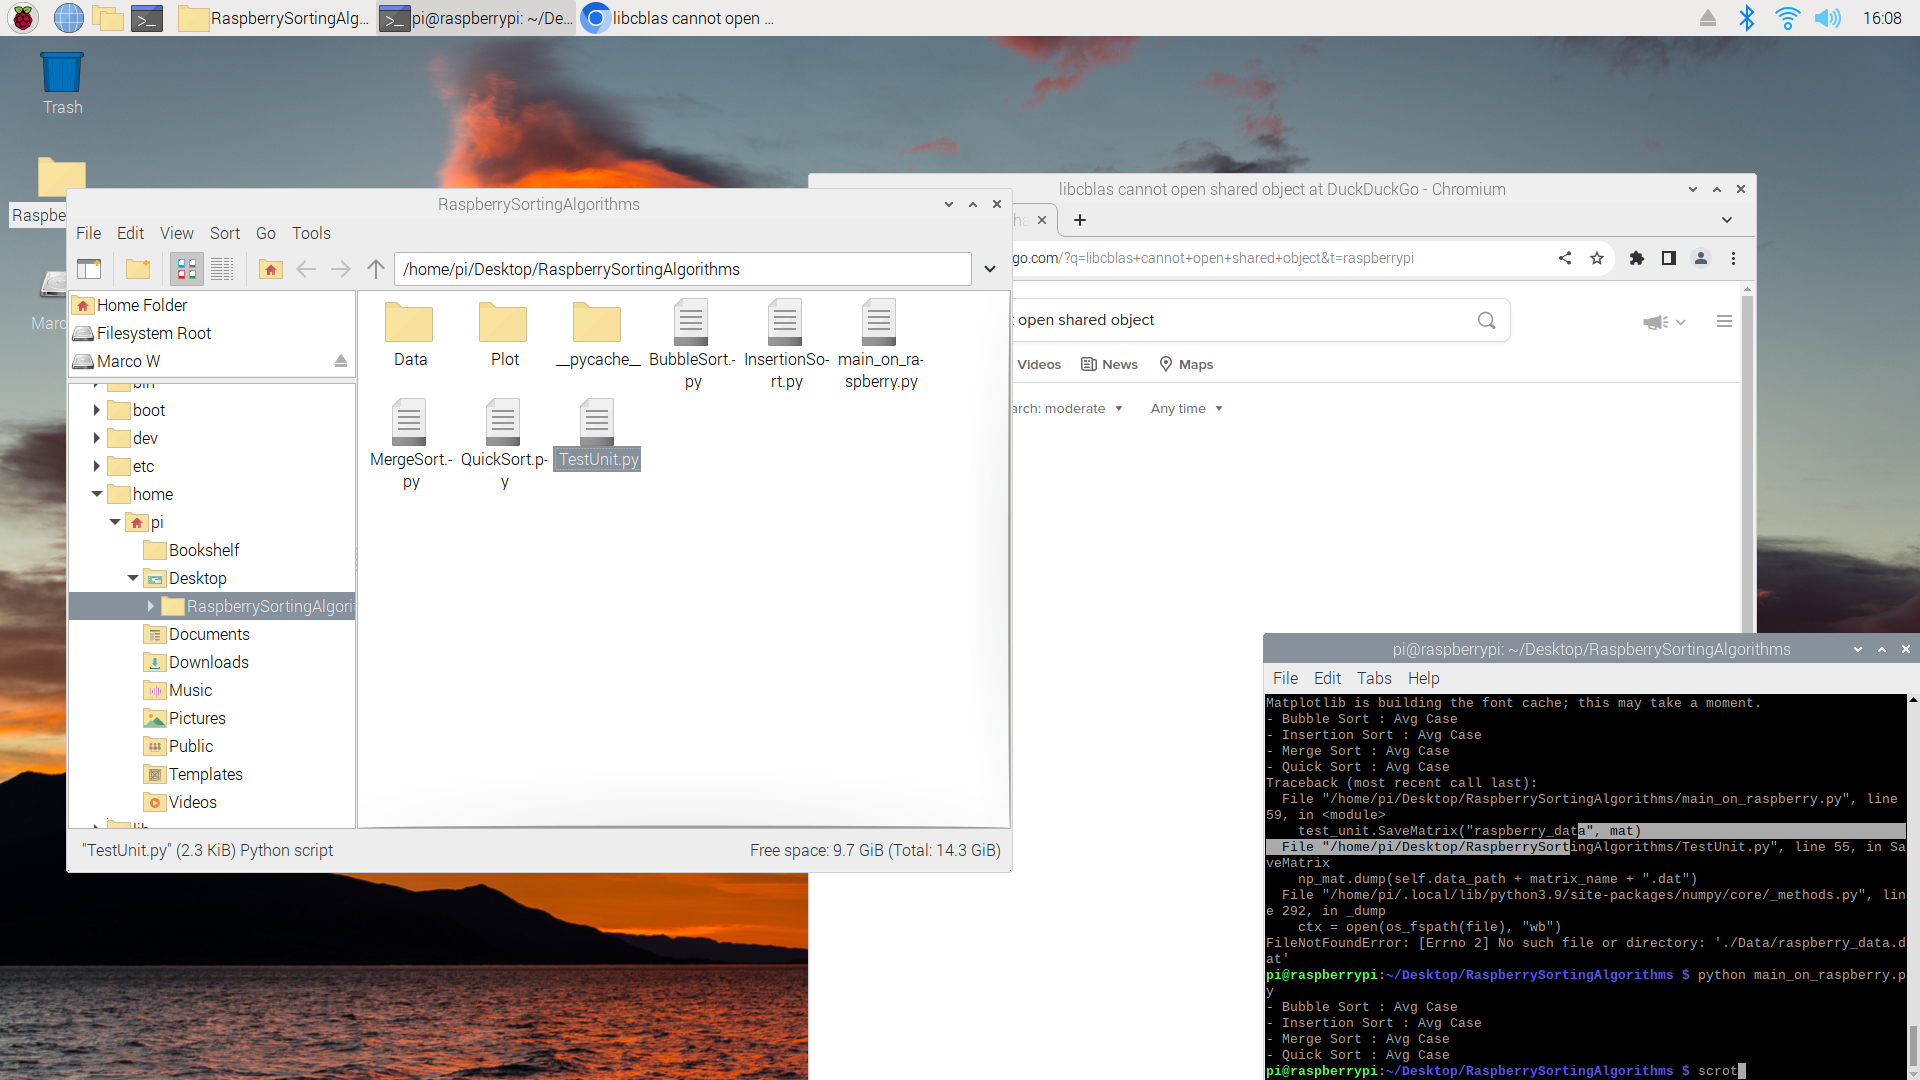
\includegraphics[width = \textwidth]{./Imgs/RaspberryScreenshot.png}
				\caption{Screenshot del lavoro svolto sulla piattaforma Raspberry}
			\end{subfigure}
  
		\end{figure}
	
	

\end{document}